\section{Five Parameter Solar Cell Model}\label{sec:five_parameter_solar_cell_model}

\subsection{Model Introduction}\label{subsec:five_param_model_introduction}

\begin{figure}[h]
    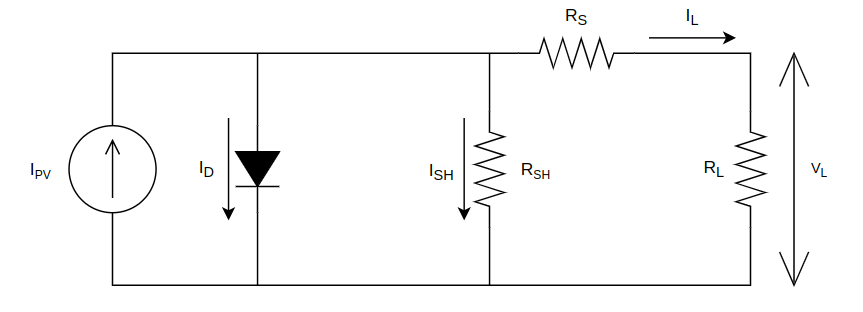
\includegraphics[width=\textwidth]{solar_cell_five_parameter_model.png}
    \caption{Five Parameter, or Full Single Diode Model of a Solar Cell}
    \label{fig:single_diode_model_with_resistances}
\end{figure}

The most common model for solar cells is the five parameter solar cell model,
shown in Figure~\ref{fig:single_diode_model_with_resistances}. This is the
complete form of the single diode model discussed in the previous section,
Section~\ref{sec:three_parameter_solar_cell_model}. There are two added
components/parameters: a series resistance \ac{RS} and shunt resistance
\ac{RSH}, whose primary role is to alter the shape of the knee-bend in the I-V
curve. As such, this model generall improves upon the main flaw of the three
parameter solar cell model, that o overshooting the maximum power point.

In the following subsections, we discuss the two added parameters and their
specific effects on the model.

\subsection{Shunt Resistance}\label{subsec:five_param_shunt_resistance}

\begin{figure}[h]
    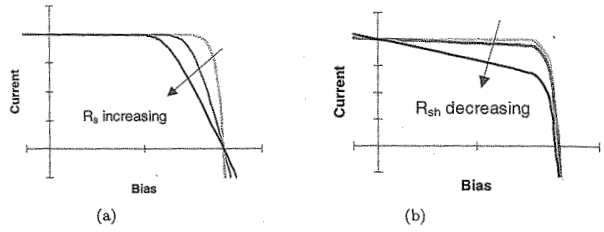
\includegraphics[width=\textwidth]{series_shunt_resistance.png}
    \caption{Effect of Series (a) and Shunt Resistance (b) on \ac{I-V} Curve}
    \label{fig:series_shunt_resistance}
\end{figure}

As shown in Figure~\ref{fig:series_shunt_resistance} from Nelson~\cite{nelson},
as the shunt resistance \ac{RSH} decreases the top of the knee-bend of the
\ac{I-V} curve will be forced down. At low values of shunt resistance (at the
order of $10$ $\si{\ohm}$), the knee-bend will be pushed down so much that the
curve becomes a straight light. At high values of shunt resistance, (at the
order of $100$ $\si{\ohm}$), the curve converges to some fixed maximum bend
constrained by other parameters of the model. This relationship is generally
considered logarithmic.

The \ac{ISH} is present in the simple form of the model as
Equation~\ref{eq:cell_output_current_3}. Assuming that the series resistance is
negligible ($0$), we can determine that \ac{ISH} is a function of the \ac{RSH}
and the voltage across the cell \ac{V}, shown in
Equation~\ref{eq:cell_output_current_4}.

\begin{equation}
    I_L = I_{PV} - I_D - I_{SH}
    \equnit{\si{\ampere}}
    \label{eq:cell_output_current_3}
\end{equation}

\begin{equation}
    I_L = I_{PV} - I_D - \frac{V}{R_{SH}}
    \equnit{\si{\ampere}}
    \label{eq:cell_output_current_4}
\end{equation}




\subsection{Series Resistance}\label{subsec:five_param_series_resistance}



